\documentclass[11pt, a4paper]{article} 

\usepackage[utf8]{inputenc}  

\usepackage{caption}  			% provides commands for handling caption sizes etc.
%\usepackage[a4paper, left=25mm, right=20mm, top=25mm, bottom=20mm]{geometry}		 % to easily change margin widths: https://www.sharelatex.com/learn/Page_size_and_margins

\usepackage{etoolbox}    % for conditional evaluations!
\usepackage[bottom]{footmisc}  % I love footnotes! And they should be down at the bottom of the page!
\usepackage{graphicx}        % when using figures and alike
\usepackage[hidelinks]{hyperref}		% for hyperreferences (links within the document: references, figures, tables, citations)

\usepackage{euler}     % a math font, only for equations and alike; call BEFORE changing the main font; alternatives: mathptmx, fourier, 
%\usepackage{gentium} % for a different font; you can also try: cantarell, charter, libertine, gentium, bera, ... http://tex.stackexchange.com/questions/59403/what-font-packages-are-installed-in-tex-live

%------------------------------------------------------------------------------------------------------
%------- text size settings --------------
\setlength{\textwidth}{16cm}% 
\setlength{\textheight}{25cm} %23 
%(these values were used to fill the page more fully and thus reduce the number of pages!)
\setlength{\topmargin}{-1.5cm} %0
\setlength{\footskip}{1cm} %
%\setlength{\hoffset}{0cm} %
\setlength{\oddsidemargin}{1cm}%
\setlength{\evensidemargin}{-.5cm}%
\setlength{\parskip}{0cm} % Abstand zwischen Absätzen
% ----------------------------------------------------------------
\renewcommand{\textfraction}{0.1} % allows more space to graphics in float
\renewcommand{\topfraction}{0.85}
%\renewcommand{\bottomfraction}{0.65}
\renewcommand{\floatpagefraction}{0.70}


\frenchspacing %http://texwelt.de/wissen/fragen/1154/was-ist-french-spacing-was-macht-frenchspacing
%------------------------------------------------------------------------------------------------------
%------------------------------------------------------------------------------------------------------

\usepackage{Sweave}
\begin{document}
\Sconcordance{concordance:sweave_document_TB.tex:sweave_document_TB.Rnw:%
<<<<<<< Updated upstream
1 39 1 1 0 22 1 1 8 4 1 1 7 1 2 9 1 2 2 4 1 1 4 1 1 1 4 20 1}
=======
1 39 1 1 0 24 1 1 7 1 2 6 1 1 4 1 2 3 1}
>>>>>>> Stashed changes

\begin{Schunk}
\begin{Soutput}
'data.frame':	2220 obs. of  23 variables:
 $ row.ID                 : int  1 2 3 4 5 6 7 8 9 10 ...
 $ study.ID               : int  1 1 1 1 1 1 1 1 1 1 ...
 $ continent              : Factor w/ 4 levels "AF","AS","CA",..: 4 4 4 4 4 4 4 4 4 4 ...
 $ taxon                  : Factor w/ 4 levels "a","b","m","p": 1 1 1 1 1 1 1 1 1 1 ...
 $ taxon.specific         : Factor w/ 359 levels "",">3 habitats used",..: 150 150 148 148 159 159 211 211 224 224 ...
 $ taxon.arthropod.order  : Factor w/ 4 levels "","c","h","l": 4 4 1 1 1 1 4 4 3 3 ...
 $ taxon.mammal.group     : Factor w/ 6 levels "","b","l","p",..: 1 1 1 1 1 1 1 1 1 1 ...
 $ taxon.forest.generalist: Factor w/ 3 levels "","f","g": 1 1 1 1 1 1 1 1 1 1 ...
 $ metric                 : Factor w/ 5 levels "abu","com","dem",..: 5 5 5 5 5 5 5 5 5 5 ...
 $ metric.specific        : Factor w/ 497 levels "Above-ground biomass (t)",..: 316 316 314 314 330 330 323 323 324 324 ...
 $ disturbance            : Factor w/ 12 levels "abn","agf","agr",..: 9 10 9 10 9 10 9 10 9 10 ...
 $ disturbance.specific   : Factor w/ 241 levels "22 year old selectively logged forests",..: 172 186 172 186 172 186 172 186 172 186 ...
 $ matrix                 : Factor w/ 5 levels "agr","dis","nat",..: 3 3 3 3 3 3 3 3 3 3 ...
 $ distance.p.d           : Factor w/ 47 levels "0.1","0.25","0.3",..: 8 8 8 8 8 8 8 8 8 8 ...
 $ time                   : Factor w/ 39 levels "0","0.5","0.75",..: 30 14 30 14 30 14 30 14 30 14 ...
 $ effect.direction       : Factor w/ 2 levels "d","p": 2 2 2 2 2 2 2 2 2 2 ...
 $ p.mean                 : Factor w/ 918 levels "0","0.005766667",..: 209 209 425 425 324 324 205 205 352 352 ...
 $ p.sd                   : Factor w/ 896 levels "0","0.00311127",..: 714 714 564 564 549 549 766 766 395 395 ...
 $ p.n                    : int  5 5 5 5 5 5 5 5 5 5 ...
 $ d.mean                 : Factor w/ 1450 levels "0","0.00049",..: 1134 1382 704 766 415 511 344 382 663 614 ...
 $ d.sd                   : Factor w/ 1483 levels "0","0.001159655",..: 1018 1026 652 853 674 832 1322 1395 895 830 ...
 $ d.n                    : int  5 5 5 5 5 5 5 5 5 5 ...
 $ hedges.g.              : Factor w/ 2158 levels "-0.000585762",..: 1543 1147 73 126 804 57 158 195 80 53 ...
\end{Soutput}
\begin{Soutput}
     row.ID          study.ID      continent taxon      taxon.specific
 Min.   :   1.0   Min.   :  1.00   AF:287    a:593             : 391  
 1st Qu.: 555.8   1st Qu.: 20.00   AS:608    b:529   trees     : 181  
 Median :1110.5   Median : 58.00   CA:416    m:347   bat       : 124  
 Mean   :1110.5   Mean   : 61.30   SA:909    p:751   tree      :  57  
 3rd Qu.:1665.2   3rd Qu.: 95.25                     harvestman:  46  
 Max.   :2220.0   Max.   :138.00                     shrew     :  46  
                                                     (Other)   :1375  
 taxon.arthropod.order taxon.mammal.group taxon.forest.generalist metric   
  :1777                 :1873              :2013                  abu:869  
 c: 173                b: 177             f: 149                  com:113  
 h: 136                l:   9             g:  58                  dem:108  
 l: 134                p:  13                                     for:270  
                       s:  98                                     ric:860  
                       u:  50                                              
                                                                           
                                              metric.specific  disturbance 
 Mean species richness                                : 100   sec    :687  
 Mean density (stems/ha)                              :  92   sel    :355  
 Mean abundance                                       :  52   pla    :212  
 Mean estimated species richness (jackknife estimator):  47   agr    :191  
 Average number of individuals captured per site      :  46   agf    :157  
 Density (individuals/km^2)                           :  46   shd    :152  
 (Other)                                              :1837   (Other):466  
                                                   disturbance.specific  matrix    
 Secondary forest                                            : 202      agr : 125  
 Secondary forests                                           : 144      dis :  61  
 selectively logged forest                                   :  62      nat :1557  
 second growth                                               :  59      pas : 147  
 Reduced-impact logged forest                                :  53      pla :  71  
 Disturbed forest sites (high pressure of biomass extraction):  41      NA's: 259  
 (Other)                                                     :1659                 
  distance.p.d       time     effect.direction     p.mean          p.sd     
 2.5    : 178   0      :360   d: 180           0      :  50   0      :  84  
 2      : 149   1      :108   p:2040           0.2    :  14   0.4    :  26  
 1.2    : 101   5      :107                    3.26   :  12   1      :  18  
 1.5    :  85   15     :106                    35.14  :  12   3      :  16  
 1      :  69   12     : 95                    1.9    :  11   0.5    :  15  
 (Other): 637   (Other):648                    24.9   :  11   1.3    :  15  
 NA's   :1001   NA's   :796                    (Other):2110   (Other):2046  
      p.n             d.mean          d.sd           d.n                hedges.g.   
 Min.   : 2.000   0.2    :  18   0.5    :  32   Min.   : 2.000   0           :  15  
 1st Qu.: 3.000   0.3    :  17   0      :  30   1st Qu.: 3.000   -0.614875462:   5  
 Median : 4.000   0.8    :  14   1      :  19   Median : 4.000   -0.472727274:   3  
 Mean   : 5.771   0.25   :  13   4      :  18   Mean   : 5.212   -0.571428572:   3  
 3rd Qu.: 6.000   0.5    :  13   1.5    :  15   3rd Qu.: 6.000   -0.652713952:   3  
 Max.   :50.000   0.1    :  12   0.2    :  12   Max.   :50.000   -1.019367933:   3  
                  (Other):2133   (Other):2094                    (Other)     :2188  
\end{Soutput}
\begin{Soutput}
     row.ID          study.ID     continent taxon   distance.p.d          time   
 Min.   :  14.0   Min.   :  1.0   AF: 5     a: 0   2      : 4    0          : 4  
 1st Qu.: 706.5   1st Qu.: 27.5   AS:13     b:38   2.5    : 3    1          : 3  
 Median :1109.0   Median : 59.0   CA: 5     m: 0   1.2    : 2    5          : 3  
 Mean   :1138.7   Mean   : 62.5   SA:15     p: 0   0.3    : 1    0.833333333: 2  
 3rd Qu.:1526.5   3rd Qu.: 88.5                    1      : 1    30         : 2  
 Max.   :2217.0   Max.   :138.0                    (Other): 9    (Other)    :12  
                                                   NA's   :18    NA's       :12  
 effect.direction     p.mean           p.sd            p.n             d.mean      
 d: 3             Min.   :  4.0   Min.   :  3.0   Min.   : 2.000   Min.   :   4.0  
 p:35             1st Qu.:331.5   1st Qu.:262.0   1st Qu.: 3.000   1st Qu.: 332.8  
                  Median :584.5   Median :356.0   Median : 4.500   Median : 805.0  
                  Mean   :544.7   Mean   :448.9   Mean   : 7.368   Mean   : 736.9  
                  3rd Qu.:764.5   3rd Qu.:700.5   3rd Qu.: 6.000   3rd Qu.:1066.8  
                  Max.   :851.0   Max.   :879.0   Max.   :50.000   Max.   :1434.0  
                                                                                   
      d.sd             d.n           hedges.g.   
 Min.   :   3.0   Min.   : 2.000   Min.   :  11  
 1st Qu.: 322.2   1st Qu.: 3.000   1st Qu.: 408  
 Median : 673.5   Median : 4.500   Median :1198  
 Mean   : 686.4   Mean   : 6.263   Mean   :1076  
 3rd Qu.: 998.5   3rd Qu.: 6.000   3rd Qu.:1585  
 Max.   :1462.0   Max.   :50.000   Max.   :2141  
\end{Soutput}
\begin{Soutput}
Fixed-Effects Model (k = 38)

Test for Heterogeneity: 
Q(df = 37) = 51.0598, p-val = 0.0619

Model Results:

estimate       se     zval     pval    ci.lb    ci.ub          
 -0.3194   0.0947  -3.3723   0.0007  -0.5051  -0.1338      *** 

---
Signif. codes:  0 ‘***’ 0.001 ‘**’ 0.01 ‘*’ 0.05 ‘.’ 0.1 ‘ ’ 1 
\end{Soutput}
\begin{Soutput}
Random-Effects Model (k = 38; tau^2 estimator: REML)

tau^2 (estimated amount of total heterogeneity): 0.1368 (SE = 0.1185)
tau (square root of estimated tau^2 value):      0.3699
I^2 (total heterogeneity / total variability):   27.22%
H^2 (total variability / sampling variability):  1.37

Test for Heterogeneity: 
Q(df = 37) = 47.0470, p-val = 0.1246

Model Results:

estimate       se     zval     pval    ci.lb    ci.ub          
 -0.2833   0.1223  -2.3170   0.0205  -0.5230  -0.0437        * 

---
Signif. codes:  0 ‘***’ 0.001 ‘**’ 0.01 ‘*’ 0.05 ‘.’ 0.1 ‘ ’ 1 
\end{Soutput}
\end{Schunk}

\title{Appendix}
\author{Torfinn Belbo \& Carolina Wackerhagen}

\date{\today}

\maketitle 

We created an appendix of meta-analysis paper. To be able to visualize the output, we used an example dataset taken from Gibson et al. 2011.

The dataset to be working with should be named ``data.sub''. The conducted analysis using the function rma from the metafor pacakge should be renamed as such: rma of a random effects model should be named ``rma.RE'' and an rma of a fixed effects model should be named ``rma.FE'' in order for the automatisation to work. IF a meta-regression has been conducted, it should be called ``rma.RE.meta'' or ``rma.FE.meta'' respectively. Other than that, the metafor package in R needs to be installed.  

For creating an appendix with an unkown dataset... 

\begin{figure}
\captionsetup{width =0.6\textwidth
\centering
\begin{Schunk}
\begin{Soutput}
function (x, annotate = TRUE, addfit = TRUE, addcred = FALSE, 
    showweight = FALSE, xlim, alim, clim, ylim, at, steps = 5, 
    level = x$level, digits = 2, refline = 0, xlab, slab, mlab, 
    ilab, ilab.xpos, ilab.pos, order, transf, atransf, targs, 
    rows, efac = 1, pch = 15, psize, col, border, lty, cex, cex.lab, 
    cex.axis, ...) 
{
    if (!is.element("rma", class(x))) 
        stop("Argument 'x' must be an object of class \"rma\".")
    na.act <- getOption("na.action")
    if (!is.element(na.act, c("na.omit", "na.exclude", "na.fail", 
        "na.pass"))) 
        stop("Unknown 'na.action' specified under options().")
    if (missing(transf)) 
        transf <- FALSE
    if (missing(atransf)) 
        atransf <- FALSE
    transf.char <- deparse(substitute(transf))
    atransf.char <- deparse(substitute(atransf))
    if (transf.char != "FALSE" && atransf.char != "FALSE") 
        stop("Use either 'transf' or 'atransf' to specify a transformation (not both).")
    if (missing(targs)) 
        targs <- NULL
    if (missing(at)) 
        at <- NULL
    if (missing(ilab)) 
        ilab <- NULL
    if (missing(ilab.xpos)) 
        ilab.xpos <- NULL
    if (missing(ilab.pos)) 
        ilab.pos <- NULL
    if (missing(order)) 
        order <- NULL
    if (missing(psize)) 
        psize <- NULL
    if (missing(cex)) 
        cex <- NULL
    if (missing(cex.lab)) 
        cex.lab <- NULL
    if (missing(cex.axis)) 
        cex.axis <- NULL
    if (x$int.only) {
        if (missing(col)) {
            col <- c("black", "gray50")
        }
        else {
            if (length(col) == 1L) 
                col <- c(col, "gray50")
        }
        if (missing(border)) 
            border <- "black"
    }
    else {
        if (missing(col)) 
            col <- "gray"
        if (missing(border)) 
            border <- "gray"
    }
    if (missing(lty)) {
        lty <- c("solid", "dotted")
    }
    else {
        if (length(lty) == 1L) 
            lty <- c(lty, "dotted")
    }
    measure <- x$measure
    if (is.element("rma.glmm", class(x)) && showweight) 
        stop("Option 'showweight=TRUE' currently not possible for 'rma.glmm' objects. Sorry!")
    if (length(digits) == 1L) 
        digits <- c(digits, digits)
    alpha <- ifelse(level > 1, (100 - level)/100, 1 - level)
    yi <- x$yi.f
    vi <- x$vi.f
    X <- x$X.f
    k <- length(yi)
    if (missing(slab)) {
        if (x$slab.null) {
            slab <- paste("Study ", x$slab)
        }
        else {
            slab <- x$slab
        }
    }
    if (length(yi) != length(slab)) 
        stop("Number of outcomes does not correspond to the length of the slab argument.")
    if (is.vector(ilab)) 
        ilab <- cbind(ilab)
    if (length(pch) == 1L) 
        pch <- rep(pch, k)
    if (length(pch) != length(yi)) 
        stop("Number of outcomes does not correspond to the length of the pch argument.")
    options(na.action = "na.pass")
    if (x$int.only) {
        pred <- fitted(x)
        pred.ci.lb <- rep(NA_real_, k)
        pred.ci.ub <- rep(NA_real_, k)
    }
    else {
        temp <- predict(x, level = level)
        pred <- temp$pred
        if (addcred) {
            pred.ci.lb <- temp$cr.lb
            pred.ci.ub <- temp$cr.ub
        }
        else {
            pred.ci.lb <- temp$ci.lb
            pred.ci.ub <- temp$ci.ub
        }
    }
    if (is.element("rma.glmm", class(x))) {
        weights <- NULL
    }
    else {
        weights <- weights(x)
    }
    options(na.action = na.act)
    if (!is.null(psize)) {
        if (length(psize) == 1L) 
            psize <- rep(psize, k)
        if (length(psize) != length(yi)) 
            stop("Number of outcomes does not correspond to the length of the psize argument.")
    }
    if (!is.null(order)) {
        if (is.character(order)) {
            if (length(order) != 1) 
                stop("Incorrect length of order argument.")
            if (order == "obs") 
                sort.vec <- order(yi)
            if (order == "fit") 
                sort.vec <- order(pred)
            if (order == "prec") 
                sort.vec <- order(vi, yi)
            if (order == "resid") 
                sort.vec <- order(yi - pred, yi)
            if (order == "rstandard") 
                sort.vec <- order(rstandard(x)$z, yi)
            if (order == "abs.resid") 
                sort.vec <- order(abs(yi - pred), yi)
            if (order == "abs.rstandard") 
                sort.vec <- order(abs(rstandard(x)$z), yi)
        }
        else {
            sort.vec <- order
        }
        yi <- yi[sort.vec]
        vi <- vi[sort.vec]
        X <- X[sort.vec, , drop = FALSE]
        slab <- slab[sort.vec]
        ilab <- ilab[sort.vec, , drop = FALSE]
        pred <- pred[sort.vec]
        pred.ci.lb <- pred.ci.lb[sort.vec]
        pred.ci.ub <- pred.ci.ub[sort.vec]
        weights <- weights[sort.vec]
        pch <- pch[sort.vec]
        psize <- psize[sort.vec]
    }
    k <- length(yi)
    if (missing(rows)) {
        rows <- k:1
    }
    else {
        if (length(rows) == 1L) {
            rows <- rows:(rows - k + 1)
        }
    }
    if (length(rows) != length(yi)) 
        stop("Number of outcomes does not correspond to the length of the rows argument.")
    yi <- yi[k:1]
    vi <- vi[k:1]
    X <- X[k:1, , drop = FALSE]
    slab <- slab[k:1]
    ilab <- ilab[k:1, , drop = FALSE]
    pred <- pred[k:1]
    pred.ci.lb <- pred.ci.lb[k:1]
    pred.ci.ub <- pred.ci.ub[k:1]
    weights <- weights[k:1]
    pch <- pch[k:1]
    psize <- psize[k:1]
    rows <- rows[k:1]
    yiviX.na <- is.na(cbind(yi, vi, X))
    if (any(yiviX.na)) {
        not.na <- apply(yiviX.na, MARGIN = 1, sum) == 0L
        if (na.act == "na.omit") {
            yi <- yi[not.na]
            vi <- vi[not.na]
            X <- X[not.na, , drop = FALSE]
            slab <- slab[not.na]
            ilab <- ilab[not.na, , drop = FALSE]
            pred <- pred[not.na]
            pred.ci.lb <- pred.ci.lb[not.na]
            pred.ci.ub <- pred.ci.ub[not.na]
            weights <- weights[not.na]
            pch <- pch[not.na]
            psize <- psize[not.na]
            rows.new <- rows
            rows.na <- rows[!not.na]
            for (j in seq_len(length(rows.na))) {
                rows.new[rows >= rows.na[j]] <- rows.new[rows >= 
                  rows.na[j]] - 1
            }
            rows <- rows.new[not.na]
        }
        if (na.act == "na.fail") 
            stop("Missing values in results.")
    }
    k <- length(yi)
    ci.lb <- yi - qnorm(alpha/2, lower.tail = FALSE) * sqrt(vi)
    ci.ub <- yi + qnorm(alpha/2, lower.tail = FALSE) * sqrt(vi)
    if (is.function(transf)) {
        if (is.null(targs)) {
            yi <- sapply(yi, transf)
            ci.lb <- sapply(ci.lb, transf)
            ci.ub <- sapply(ci.ub, transf)
            pred <- sapply(pred, transf)
            pred.ci.lb <- sapply(pred.ci.lb, transf)
            pred.ci.ub <- sapply(pred.ci.ub, transf)
        }
        else {
            yi <- sapply(yi, transf, targs)
            ci.lb <- sapply(ci.lb, transf, targs)
            ci.ub <- sapply(ci.ub, transf, targs)
            pred <- sapply(pred, transf, targs)
            pred.ci.lb <- sapply(pred.ci.lb, transf, targs)
            pred.ci.ub <- sapply(pred.ci.ub, transf, targs)
        }
    }
    ci.bounds <- cbind(ci.lb, ci.ub)
    rev.order <- ifelse(ci.ub < ci.lb, TRUE, FALSE)
    rev.order[is.na(rev.order)] <- FALSE
    ci.bounds[rev.order, ] <- ci.bounds[rev.order, 2:1]
    ci.lb <- ci.bounds[, 1]
    ci.ub <- ci.bounds[, 2]
    pred.ci.bounds <- cbind(pred.ci.lb, pred.ci.ub)
    rev.order <- ifelse(pred.ci.ub < pred.ci.lb, TRUE, FALSE)
    rev.order[is.na(rev.order)] <- FALSE
    pred.ci.bounds[rev.order, ] <- pred.ci.bounds[rev.order, 
        2:1]
    pred.ci.lb <- pred.ci.bounds[, 1]
    pred.ci.ub <- pred.ci.bounds[, 2]
    if (!missing(clim)) {
        clim <- sort(clim)
        if (length(clim) != 2L) 
            stop("Argument 'clim' must be of length 2.")
        ci.lb[ci.lb < clim[1]] <- clim[1]
        ci.ub[ci.ub > clim[2]] <- clim[2]
        pred.ci.lb[pred.ci.lb < clim[1]] <- clim[1]
        pred.ci.ub[pred.ci.ub > clim[2]] <- clim[2]
    }
    if (is.null(psize)) {
        if (is.null(weights)) {
            if (any(vi <= 0, na.rm = TRUE)) {
                psize <- rep(1, k)
            }
            else {
                wi <- 1/sqrt(vi)
                psize <- wi/sum(wi, na.rm = TRUE)
                psize <- (psize - min(psize, na.rm = TRUE))/(max(psize, 
                  na.rm = TRUE) - min(psize, na.rm = TRUE))
                psize <- (psize * 1) + 0.5
                if (all(is.na(psize))) 
                  psize <- rep(1, k)
            }
        }
        else {
            wi <- weights
            psize <- wi/sum(wi, na.rm = TRUE)
            psize <- (psize - min(psize, na.rm = TRUE))/(max(psize, 
                na.rm = TRUE) - min(psize, na.rm = TRUE))
            psize <- (psize * 1) + 0.5
            if (all(is.na(psize))) 
                psize <- rep(1, k)
        }
    }
    rng <- max(ci.ub, na.rm = TRUE) - min(ci.lb, na.rm = TRUE)
    if (annotate) {
        if (showweight) {
            plot.multp.l <- 2
            plot.multp.r <- 2
            axis.multp.l <- 0.2
            axis.multp.r <- 0.2
        }
        else {
            plot.multp.l <- 1.2
            plot.multp.r <- 1.2
            axis.multp.l <- 0.2
            axis.multp.r <- 0.2
        }
    }
    else {
        plot.multp.l <- 1.2
        plot.multp.r <- 0.4
        axis.multp.l <- 0.2
        axis.multp.r <- 0.2
    }
    if (missing(xlim)) {
        xlim <- c(min(ci.lb, na.rm = TRUE) - rng * plot.multp.l, 
            max(ci.ub, na.rm = TRUE) + rng * plot.multp.r)
        xlim <- round(xlim, digits[2])
    }
    alim.spec <- TRUE
    if (missing(alim)) {
        if (is.null(at)) {
            alim <- range(pretty(x = c(min(ci.lb, na.rm = TRUE), 
                max(ci.ub, na.rm = TRUE)), n = steps - 1))
            alim.spec <- FALSE
        }
        else {
            alim <- range(at)
        }
    }
    alim <- sort(alim)
    xlim <- sort(xlim)
    if (xlim[1] > min(yi, na.rm = TRUE)) {
        xlim[1] <- min(yi, na.rm = TRUE)
    }
    if (xlim[2] < max(yi, na.rm = TRUE)) {
        xlim[2] <- max(yi, na.rm = TRUE)
    }
    if (alim[1] > min(yi, na.rm = TRUE)) {
        alim[1] <- min(yi, na.rm = TRUE)
    }
    if (alim[2] < max(yi, na.rm = TRUE)) {
        alim[2] <- max(yi, na.rm = TRUE)
    }
    if (alim[1] < xlim[1]) {
        xlim[1] <- alim[1]
    }
    if (alim[2] > xlim[2]) {
        xlim[2] <- alim[2]
    }
    if (missing(ylim)) {
        if (x$int.only && addfit) {
            ylim <- c(-1.5, k + 3)
        }
        else {
            ylim <- c(0.5, k + 3)
        }
    }
    else {
        ylim <- sort(ylim)
    }
    if (is.null(at)) {
        if (alim.spec) {
            at <- seq(from = alim[1], to = alim[2], length.out = steps)
        }
        else {
            at <- pretty(x = c(min(ci.lb, na.rm = TRUE), max(ci.ub, 
                na.rm = TRUE)), n = steps - 1)
        }
    }
    else {
        at[at < alim[1]] <- alim[1]
        at[at > alim[2]] <- alim[2]
        at <- unique(at)
    }
    at.lab <- at
    if (is.function(atransf)) {
        if (is.null(targs)) {
            at.lab <- formatC(sapply(at.lab, atransf), digits = digits[2], 
                format = "f")
        }
        else {
            at.lab <- formatC(sapply(at.lab, atransf, targs), 
                digits = digits[2], format = "f")
        }
    }
    else {
        at.lab <- formatC(at.lab, digits = digits[2], format = "f")
    }
    par.mar <- par("mar")
    par.mar.adj <- par.mar - c(0, 3, 1, 1)
    par.mar.adj[par.mar.adj < 0] <- 0
    par(mar = par.mar.adj)
    on.exit(par(mar = par.mar))
    plot(NA, NA, xlim = xlim, ylim = ylim, xlab = "", ylab = "", 
        yaxt = "n", xaxt = "n", xaxs = "i", bty = "n", ...)
    abline(h = ylim[2] - 2, ...)
    par.usr <- par("usr")
    height <- par.usr[4] - par.usr[3]
    lheight <- strheight("O")
    cex.adj <- ifelse(k * lheight > height * 0.8, height/(1.25 * 
        k * lheight), 1)
    if (is.null(cex)) {
        cex <- par("cex") * cex.adj
    }
    else {
        if (is.null(cex.lab)) 
            cex.lab <- cex
        if (is.null(cex.axis)) 
            cex.axis <- cex
    }
    if (is.null(cex.lab)) 
        cex.lab <- par("cex") * cex.adj
    if (is.null(cex.axis)) 
        cex.axis <- par("cex") * cex.adj
    if (addfit && !x$int.only) {
        for (i in seq_len(k)) {
            if (is.na(pred[i])) 
                next
            polygon(x = c(max(pred.ci.lb[i], alim[1]), pred[i], 
                min(pred.ci.ub[i], alim[2]), pred[i]), y = c(rows[i], 
                rows[i] + (height/100) * cex * efac, rows[i], 
                rows[i] - (height/100) * cex * efac), col = col, 
                border = border, ...)
        }
    }
    if (addfit && x$int.only) {
        if (is.element("rma.mv", class(x)) && x$withG && is.element(x$struct, 
            c("HCS", "UN", "HAR"))) {
            if (!is.logical(addcred)) {
                temp <- predict(x, level = level, tau2.levels = addcred[1])
                addcred <- TRUE
            }
            else {
                if (addcred) {
                  stop("Need to specify the level of the inner factor via the 'addcred' argument.")
                }
                else {
                  temp <- predict(x, level = level, tau2.levels = 1)
                }
            }
        }
        else {
            temp <- predict(x, level = level)
        }
        b <- temp$pred
        b.ci.lb <- temp$ci.lb
        b.ci.ub <- temp$ci.ub
        b.cr.lb <- temp$cr.lb
        b.cr.ub <- temp$cr.ub
        if (is.function(transf)) {
            if (is.null(targs)) {
                b <- sapply(b, transf)
                b.ci.lb <- sapply(b.ci.lb, transf)
                b.ci.ub <- sapply(b.ci.ub, transf)
                b.cr.lb <- sapply(b.cr.lb, transf)
                b.cr.ub <- sapply(b.cr.ub, transf)
            }
            else {
                b <- sapply(b, transf, targs)
                b.ci.lb <- sapply(b.ci.lb, transf, targs)
                b.ci.ub <- sapply(b.ci.ub, transf, targs)
                b.cr.lb <- sapply(b.cr.lb, transf, targs)
                b.cr.ub <- sapply(b.cr.ub, transf, targs)
            }
        }
        b.ci.bounds <- cbind(b.ci.lb, b.ci.ub)
        rev.order <- ifelse(b.ci.ub < b.ci.lb, TRUE, FALSE)
        rev.order[is.na(rev.order)] <- FALSE
        b.ci.bounds[rev.order, ] <- b.ci.bounds[rev.order, 2:1]
        b.ci.lb <- b.ci.bounds[, 1]
        b.ci.ub <- b.ci.bounds[, 2]
        b.cr.bounds <- cbind(b.cr.lb, b.cr.ub)
        rev.order <- ifelse(b.cr.ub < b.cr.lb, TRUE, FALSE)
        rev.order[is.na(rev.order)] <- FALSE
        b.cr.bounds[rev.order, ] <- b.cr.bounds[rev.order, 2:1]
        b.cr.lb <- b.cr.bounds[, 1]
        b.cr.ub <- b.cr.bounds[, 2]
        if (!missing(clim)) {
            b.ci.lb[b.ci.lb < clim[1]] <- clim[1]
            b.ci.ub[b.ci.ub > clim[2]] <- clim[2]
            b.cr.lb[b.cr.lb < clim[1]] <- clim[1]
            b.cr.ub[b.cr.ub > clim[2]] <- clim[2]
        }
        if (x$method != "FE" && addcred) {
            segments(max(b.cr.lb, alim[1]), -1, min(b.cr.ub, 
                alim[2]), -1, lty = lty[2], col = col[2], ...)
            if (b.cr.lb >= alim[1]) {
                segments(b.cr.lb, -1 - (height/150) * cex * efac, 
                  b.cr.lb, -1 + (height/150) * cex * efac, col = col[2], 
                  ...)
            }
            else {
                polygon(x = c(alim[1], alim[1] + (1.4/100) * 
                  cex * (xlim[2] - xlim[1]), alim[1] + (1.4/100) * 
                  cex * (xlim[2] - xlim[1]), alim[1]), y = c(-1, 
                  -1 + (height/150) * cex * efac, -1 - (height/150) * 
                    cex * efac, -1), col = col[2], border = col[2], 
                  ...)
            }
            if (b.cr.ub <= alim[2]) {
                segments(b.cr.ub, -1 - (height/150) * cex * efac, 
                  b.cr.ub, -1 + (height/150) * cex * efac, col = col[2], 
                  ...)
            }
            else {
                polygon(x = c(alim[2], alim[2] - (1.4/100) * 
                  cex * (xlim[2] - xlim[1]), alim[2] - (1.4/100) * 
                  cex * (xlim[2] - xlim[1]), alim[2]), y = c(-1, 
                  -1 + (height/150) * cex * efac, -1 - (height/150) * 
                    cex * efac, -1), col = col[2], border = col[2], 
                  ...)
            }
        }
        polygon(x = c(b.ci.lb, b, b.ci.ub, b), y = c(-1, -1 + 
            (height/100) * cex * efac, -1, -1 - (height/100) * 
            cex * efac), col = col[1], border = border, ...)
        if (missing(mlab)) 
            mlab <- ifelse((x$method == "FE"), "FE Model", "RE Model")
        text(xlim[1], -1, mlab, pos = 4, cex = cex, ...)
    }
    axis(side = 1, at = at, labels = at.lab, cex.axis = cex.axis, 
        ...)
    if (missing(xlab)) 
        xlab <- .setxlab(measure, transf.char, atransf.char, 
            gentype = 1)
    mtext(xlab, side = 1, at = min(at) + (max(at) - min(at))/2, 
        line = par("mgp")[1] - 0.5, cex = cex.lab, ...)
    for (i in seq_len(k)) {
        if (is.na(yi[i]) || is.na(vi)[i]) 
            next
        segments(max(ci.lb[i], alim[1]), rows[i], min(ci.ub[i], 
            alim[2]), rows[i], lty = lty[1], ...)
        if (ci.lb[i] >= alim[1]) {
            segments(ci.lb[i], rows[i] - (height/150) * cex * 
                efac, ci.lb[i], rows[i] + (height/150) * cex * 
                efac, ...)
        }
        else {
            polygon(x = c(alim[1], alim[1] + (1.4/100) * cex * 
                (xlim[2] - xlim[1]), alim[1] + (1.4/100) * cex * 
                (xlim[2] - xlim[1]), alim[1]), y = c(rows[i], 
                rows[i] + (height/150) * cex * efac, rows[i] - 
                  (height/150) * cex * efac, rows[i]), col = "black", 
                ...)
        }
        if (ci.ub[i] <= alim[2]) {
            segments(ci.ub[i], rows[i] - (height/150) * cex * 
                efac, ci.ub[i], rows[i] + (height/150) * cex * 
                efac, ...)
        }
        else {
            polygon(x = c(alim[2], alim[2] - (1.4/100) * cex * 
                (xlim[2] - xlim[1]), alim[2] - (1.4/100) * cex * 
                (xlim[2] - xlim[1]), alim[2]), y = c(rows[i], 
                rows[i] + (height/150) * cex * efac, rows[i] - 
                  (height/150) * cex * efac, rows[i]), col = "black", 
                ...)
        }
    }
    text(xlim[1], rows, slab, pos = 4, cex = cex, ...)
    if (!is.null(ilab)) {
        if (is.null(ilab.xpos)) 
            stop("Must specify 'ilab.xpos' argument when adding information with 'ilab'.")
        if (length(ilab.xpos) != NCOL(ilab)) 
            stop("Number of 'ilab' columns does not match length of 'ilab.xpos' argument.")
        for (l in seq_len(NCOL(ilab))) {
            text(ilab.xpos[l], rows, ilab[, l], pos = ilab.pos[l], 
                cex = cex, ...)
        }
    }
    if (is.numeric(refline)) 
        segments(refline, ylim[1] - 5, refline, ylim[2] - 2, 
            lty = "dotted", ...)
    if (annotate) {
        if (is.function(atransf)) {
            if (is.null(targs)) {
                if (addfit && x$int.only) {
                  annotext <- round(cbind(sapply(c(yi, b), atransf), 
                    sapply(c(ci.lb, b.ci.lb), atransf), sapply(c(ci.ub, 
                      b.ci.ub), atransf)), digits[1])
                }
                else {
                  annotext <- round(cbind(sapply(yi, atransf), 
                    sapply(ci.lb, atransf), sapply(ci.ub, atransf)), 
                    digits[1])
                }
            }
            else {
                if (addfit && x$int.only) {
                  annotext <- round(cbind(sapply(c(yi, b), atransf, 
                    targs), sapply(c(ci.lb, b.ci.lb), atransf, 
                    targs), sapply(c(ci.ub, b.ci.ub), atransf, 
                    targs)), digits[1])
                }
                else {
                  annotext <- round(cbind(sapply(yi, atransf, 
                    targs), sapply(ci.lb, atransf, targs), sapply(ci.ub, 
                    atransf, targs)), digits[1])
                }
            }
            rev.order <- ifelse(annotext[, 3] < annotext[, 2], 
                TRUE, FALSE)
            rev.order[is.na(rev.order)] <- FALSE
            annotext[rev.order, 2:3] <- annotext[rev.order, 3:2]
        }
        else {
            if (addfit && x$int.only) {
                annotext <- round(cbind(c(yi, b), c(ci.lb, b.ci.lb), 
                  c(ci.ub, b.ci.ub)), digits[1])
            }
            else {
                annotext <- round(cbind(yi, ci.lb, ci.ub), digits[1])
            }
        }
        if (showweight) {
            if (addfit && x$int.only) {
                annotext <- cbind(round(c(weights, 100), digits[1]), 
                  annotext)
            }
            else {
                annotext <- cbind(round(weights, digits[1]), 
                  annotext)
            }
            annotext <- matrix(apply(annotext, 2, format, nsmall = digits[1]), 
                ncol = 4)
            annotext <- cbind(annotext[, 1], "%    ", annotext[, 
                2], " [ ", annotext[, 3], " , ", annotext[, 4], 
                " ]")
        }
        else {
            annotext <- matrix(apply(annotext, 2, format, nsmall = digits[1]), 
                ncol = 3)
            annotext <- cbind(annotext[, 1], " [ ", annotext[, 
                2], " , ", annotext[, 3], " ]")
        }
        annotext <- apply(annotext, 1, paste, collapse = "")
        if (addfit && x$int.only) {
            text(x = xlim[2], c(rows, -1), labels = annotext, 
                pos = 2, cex = cex, ...)
        }
        else {
            text(x = xlim[2], rows, labels = annotext, pos = 2, 
                cex = cex, ...)
        }
    }
    points(yi, rows, pch = pch, cex = cex * psize, ...)
    if (x$int.only && addfit) 
        abline(h = 0, ...)
    res <- list(xlim = par("usr")[1:2], alim = alim, at = at, 
        ylim = ylim, rows = rows, cex = cex, cex.lab = cex.lab, 
        cex.axis = cex.axis)
    invisible(res)
}
<bytecode: 0x7fa326859cd0>
<environment: namespace:metafor>
\end{Soutput}
\end{Schunk}
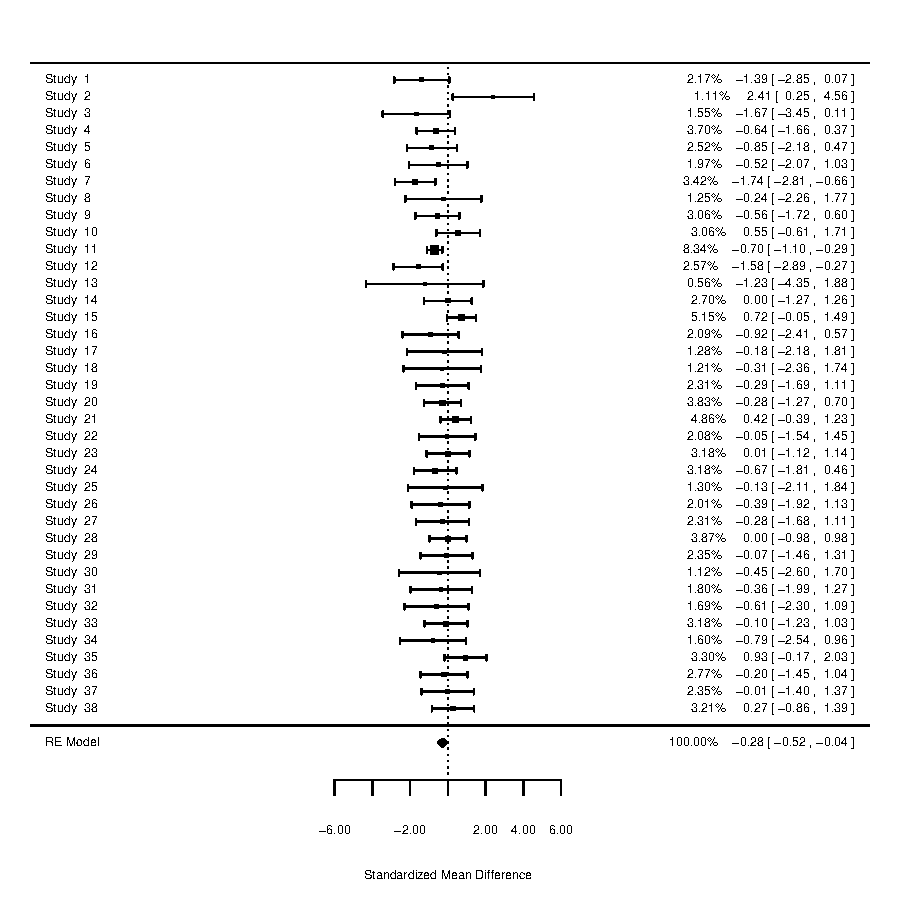
\includegraphics{sweave_document_TB-forest.re}
\caption{forest plot}
\label{forest.re}
\end{figure}

%\begin{figure}
%\begin{center}
%<<label = forest.rme, fig = TRUE, echo = FALSE, fig = TRUE, dev = "pdf">>=
%#Forest plot for the RE model
%par(mar=c(4,4,1,2))
%forest.rma(rma.RE, annotate = TRUE, cex = 0.5, showweight = TRUE) #RE model
%forest.rma
%par(mar=c(5,4,4,2))
%@
%\end{center}
%\caption{This is an example figure, exported as PDF and then, on loading, %scaled to half the text's width.}
%\end{figure}


%use  an if expression. If rma.FE = TRUE, then do the plots for FE, if not, do the plots with RE in the code. 

Forest plot of the fixed effects model...

%Causes of heterogeneity - Meta-regression p. 141
% If they did their own meta-regression, create a table with the values  obtained by the meta-regression. Include the intercept and the other moderators


%publication bias testing

%-- Fail safe n method


\end{document}
